\documentclass[1p]{elsarticle_modified}
%\bibliographystyle{elsarticle-num}

%\usepackage[colorlinks]{hyperref}
%\usepackage{abbrmath_seonhwa} %\Abb, \Ascr, \Acal ,\Abf, \Afrak
\usepackage{amsfonts}
\usepackage{amssymb}
\usepackage{amsmath}
\usepackage{amsthm}
\usepackage{scalefnt}
\usepackage{amsbsy}
\usepackage{kotex}
\usepackage{caption}
\usepackage{subfig}
\usepackage{color}
\usepackage{graphicx}
\usepackage{xcolor} %% white, black, red, green, blue, cyan, magenta, yellow
\usepackage{float}
\usepackage{setspace}
\usepackage{hyperref}

\usepackage{tikz}
\usetikzlibrary{arrows}

\usepackage{multirow}
\usepackage{array} % fixed length table
\usepackage{hhline}

%%%%%%%%%%%%%%%%%%%%%
\makeatletter
\renewcommand*\env@matrix[1][\arraystretch]{%
	\edef\arraystretch{#1}%
	\hskip -\arraycolsep
	\let\@ifnextchar\new@ifnextchar
	\array{*\c@MaxMatrixCols c}}
\makeatother %https://tex.stackexchange.com/questions/14071/how-can-i-increase-the-line-spacing-in-a-matrix
%%%%%%%%%%%%%%%

\usepackage[normalem]{ulem}

\newcommand{\msout}[1]{\ifmmode\text{\sout{\ensuremath{#1}}}\else\sout{#1}\fi}
%SOURCE: \msout is \stkout macro in https://tex.stackexchange.com/questions/20609/strikeout-in-math-mode

\newcommand{\cancel}[1]{
	\ifmmode
	{\color{red}\msout{#1}}
	\else
	{\color{red}\sout{#1}}
	\fi
}

\newcommand{\add}[1]{
	{\color{blue}\uwave{#1}}
}

\newcommand{\replace}[2]{
	\ifmmode
	{\color{red}\msout{#1}}{\color{blue}\uwave{#2}}
	\else
	{\color{red}\sout{#1}}{\color{blue}\uwave{#2}}
	\fi
}

\newcommand{\Sol}{\mathcal{S}} %segment
\newcommand{\D}{D} %diagram
\newcommand{\A}{\mathcal{A}} %arc


%%%%%%%%%%%%%%%%%%%%%%%%%%%%%5 test

\def\sl{\operatorname{\textup{SL}}(2,\Cbb)}
\def\psl{\operatorname{\textup{PSL}}(2,\Cbb)}
\def\quan{\mkern 1mu \triangleright \mkern 1mu}

\theoremstyle{definition}
\newtheorem{thm}{Theorem}[section]
\newtheorem{prop}[thm]{Proposition}
\newtheorem{lem}[thm]{Lemma}
\newtheorem{ques}[thm]{Question}
\newtheorem{cor}[thm]{Corollary}
\newtheorem{defn}[thm]{Definition}
\newtheorem{exam}[thm]{Example}
\newtheorem{rmk}[thm]{Remark}
\newtheorem{alg}[thm]{Algorithm}

\newcommand{\I}{\sqrt{-1}}
\begin{document}

%\begin{frontmatter}
%
%\title{Boundary parabolic representations of knots up to 8 crossings}
%
%%% Group authors per affiliation:
%\author{Yunhi Cho} 
%\address{Department of Mathematics, University of Seoul, Seoul, Korea}
%\ead{yhcho@uos.ac.kr}
%
%
%\author{Seonhwa Kim} %\fnref{s_kim}}
%\address{Center for Geometry and Physics, Institute for Basic Science, Pohang, 37673, Korea}
%\ead{ryeona17@ibs.re.kr}
%
%\author{Hyuk Kim}
%\address{Department of Mathematical Sciences, Seoul National University, Seoul 08826, Korea}
%\ead{hyukkim@snu.ac.kr}
%
%\author{Seokbeom Yoon}
%\address{Department of Mathematical Sciences, Seoul National University, Seoul, 08826,  Korea}
%\ead{sbyoon15@snu.ac.kr}
%
%\begin{abstract}
%We find all boundary parabolic representation of knots up to 8 crossings.
%
%\end{abstract}
%\begin{keyword}
%    \MSC[2010] 57M25 
%\end{keyword}
%
%\end{frontmatter}

%\linenumbers
%\tableofcontents
%
\newcommand\colored[1]{\textcolor{white}{\rule[-0.35ex]{0.8em}{1.4ex}}\kern-0.8em\color{red} #1}%
%\newcommand\colored[1]{\textcolor{white}{ #1}\kern-2.17ex	\textcolor{white}{ #1}\kern-1.81ex	\textcolor{white}{ #1}\kern-2.15ex\color{red}#1	}

{\Large $\underline{12n_{0568}~(K12n_{0568})}$}

\setlength{\tabcolsep}{10pt}
\renewcommand{\arraystretch}{1.6}
\vspace{1cm}\begin{tabular}{m{100pt}>{\centering\arraybackslash}m{274pt}}
\multirow{5}{120pt}{
	\centering
	\includegraphics[width=112pt]{../../../GIT/diagram.site/Diagrams/png/2657_12n_0568.png}\\
\ \ \ A knot diagram\footnotemark}&
\allowdisplaybreaks
\textbf{Linearized knot diagam} \\
\cline{2-2}
 &
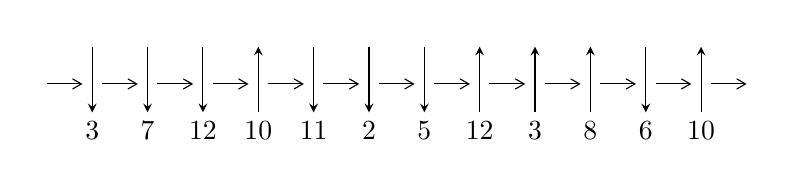
\begin{tikzpicture}[x=20pt, y=17pt]
	% nodes
	\node (C0) at (0, 0) {};
	\node (C1) at (1, 0) {};
	\node (C1U) at (1, +1) {};
	\node (C1D) at (1, -1) {3};

	\node (C2) at (2, 0) {};
	\node (C2U) at (2, +1) {};
	\node (C2D) at (2, -1) {7};

	\node (C3) at (3, 0) {};
	\node (C3U) at (3, +1) {};
	\node (C3D) at (3, -1) {12};

	\node (C4) at (4, 0) {};
	\node (C4U) at (4, +1) {};
	\node (C4D) at (4, -1) {10};

	\node (C5) at (5, 0) {};
	\node (C5U) at (5, +1) {};
	\node (C5D) at (5, -1) {11};

	\node (C6) at (6, 0) {};
	\node (C6U) at (6, +1) {};
	\node (C6D) at (6, -1) {2};

	\node (C7) at (7, 0) {};
	\node (C7U) at (7, +1) {};
	\node (C7D) at (7, -1) {5};

	\node (C8) at (8, 0) {};
	\node (C8U) at (8, +1) {};
	\node (C8D) at (8, -1) {12};

	\node (C9) at (9, 0) {};
	\node (C9U) at (9, +1) {};
	\node (C9D) at (9, -1) {3};

	\node (C10) at (10, 0) {};
	\node (C10U) at (10, +1) {};
	\node (C10D) at (10, -1) {8};

	\node (C11) at (11, 0) {};
	\node (C11U) at (11, +1) {};
	\node (C11D) at (11, -1) {6};

	\node (C12) at (12, 0) {};
	\node (C12U) at (12, +1) {};
	\node (C12D) at (12, -1) {10};
	\node (C13) at (13, 0) {};

	% arrows
	\draw[->,>={angle 60}]
	(C0) edge (C1) (C1) edge (C2) (C2) edge (C3) (C3) edge (C4) (C4) edge (C5) (C5) edge (C6) (C6) edge (C7) (C7) edge (C8) (C8) edge (C9) (C9) edge (C10) (C10) edge (C11) (C11) edge (C12) (C12) edge (C13) ;	\draw[->,>=stealth]
	(C1U) edge (C1D) (C2U) edge (C2D) (C3U) edge (C3D) (C4D) edge (C4U) (C5U) edge (C5D) (C6U) edge (C6D) (C7U) edge (C7D) (C8D) edge (C8U) (C9D) edge (C9U) (C10D) edge (C10U) (C11U) edge (C11D) (C12D) edge (C12U) ;
	\end{tikzpicture} \\
\hhline{~~} \\& 
\textbf{Solving Sequence} \\ \cline{2-2} 
 &
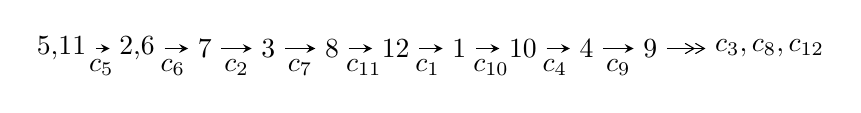
\begin{tikzpicture}[x=23pt, y=7pt]
	% node
	\node (A0) at (-1/8, 0) {5,11};
	\node (A1) at (17/16, 0) {2,6};
	\node (A2) at (17/8, 0) {7};
	\node (A3) at (25/8, 0) {3};
	\node (A4) at (33/8, 0) {8};
	\node (A5) at (41/8, 0) {12};
	\node (A6) at (49/8, 0) {1};
	\node (A7) at (57/8, 0) {10};
	\node (A8) at (65/8, 0) {4};
	\node (A9) at (73/8, 0) {9};
	\node (C1) at (1/2, -1) {$c_{5}$};
	\node (C2) at (13/8, -1) {$c_{6}$};
	\node (C3) at (21/8, -1) {$c_{2}$};
	\node (C4) at (29/8, -1) {$c_{7}$};
	\node (C5) at (37/8, -1) {$c_{11}$};
	\node (C6) at (45/8, -1) {$c_{1}$};
	\node (C7) at (53/8, -1) {$c_{10}$};
	\node (C8) at (61/8, -1) {$c_{4}$};
	\node (C9) at (69/8, -1) {$c_{9}$};
	\node (A10) at (11, 0) {$c_{3},c_{8},c_{12}$};

	% edge
	\draw[->,>=stealth]	
	(A0) edge (A1) (A1) edge (A2) (A2) edge (A3) (A3) edge (A4) (A4) edge (A5) (A5) edge (A6) (A6) edge (A7) (A7) edge (A8) (A8) edge (A9) ;
	\draw[->>,>={angle 60}]	
	(A9) edge (A10);
\end{tikzpicture} \\ 

\end{tabular} \\

\footnotetext{
The image of knot diagram is generated by the software ``\textbf{Draw programme}" developed by Andrew Bartholomew(\url{http://www.layer8.co.uk/maths/draw/index.htm\#Running-draw}), where we modified some parts for our purpose(\url{https://github.com/CATsTAILs/LinksPainter}).
}\phantom \\ \newline 
\centering \textbf{Ideals for irreducible components\footnotemark of $X_{\text{par}}$} 
 
\begin{align*}
I^u_{1}&=\langle 
3.56196\times10^{180} u^{75}-6.92402\times10^{180} u^{74}+\cdots+4.56975\times10^{180} b-7.18244\times10^{182},\\
\phantom{I^u_{1}}&\phantom{= \langle  }3.11091\times10^{181} u^{75}-7.34911\times10^{181} u^{74}+\cdots+1.32523\times10^{182} a-3.27637\times10^{183},\\
\phantom{I^u_{1}}&\phantom{= \langle  }u^{76}-3 u^{75}+\cdots+936 u+232\rangle \\
I^u_{2}&=\langle 
248830399 u^{22}+208402801 u^{21}+\cdots+79543084 b-1349697652,\\
\phantom{I^u_{2}}&\phantom{= \langle  }410409361 u^{22}+348035792 u^{21}+\cdots+79543084 a-2188204696,\;u^{23}+2 u^{22}+\cdots-8 u-8\rangle \\
\\
\end{align*}
\raggedright * 2 irreducible components of $\dim_{\mathbb{C}}=0$, with total 99 representations.\\
\footnotetext{All coefficients of polynomials are rational numbers. But the coefficients are sometimes approximated in decimal forms when there is not enough margin.}
\newpage
\renewcommand{\arraystretch}{1}
\centering \section*{I. $I^u_{1}= \langle 3.56\times10^{180} u^{75}-6.92\times10^{180} u^{74}+\cdots+4.57\times10^{180} b-7.18\times10^{182},\;3.11\times10^{181} u^{75}-7.35\times10^{181} u^{74}+\cdots+1.33\times10^{182} a-3.28\times10^{183},\;u^{76}-3 u^{75}+\cdots+936 u+232 \rangle$}
\flushleft \textbf{(i) Arc colorings}\\
\begin{tabular}{m{7pt} m{180pt} m{7pt} m{180pt} }
\flushright $a_{5}=$&$\begin{pmatrix}1\\0\end{pmatrix}$ \\
\flushright $a_{11}=$&$\begin{pmatrix}0\\u\end{pmatrix}$ \\
\flushright $a_{2}=$&$\begin{pmatrix}-0.234745 u^{75}+0.554555 u^{74}+\cdots+169.599 u+24.7231\\-0.779466 u^{75}+1.51519 u^{74}+\cdots+787.398 u+157.174\end{pmatrix}$ \\
\flushright $a_{6}=$&$\begin{pmatrix}1\\u^2\end{pmatrix}$ \\
\flushright $a_{7}=$&$\begin{pmatrix}0.498809 u^{75}-0.947197 u^{74}+\cdots-460.943 u-87.1424\\1.15577 u^{75}-2.09127 u^{74}+\cdots-1178.23 u-242.449\end{pmatrix}$ \\
\flushright $a_{3}=$&$\begin{pmatrix}0.913618 u^{75}-1.62170 u^{74}+\cdots-954.260 u-197.783\\0.641894 u^{75}-1.15647 u^{74}+\cdots-655.502 u-136.716\end{pmatrix}$ \\
\flushright $a_{8}=$&$\begin{pmatrix}-0.656963 u^{75}+1.14407 u^{74}+\cdots+717.288 u+155.306\\1.15577 u^{75}-2.09127 u^{74}+\cdots-1178.23 u-242.449\end{pmatrix}$ \\
\flushright $a_{12}=$&$\begin{pmatrix}- u\\- u^3+u\end{pmatrix}$ \\
\flushright $a_{1}=$&$\begin{pmatrix}0.631741 u^{75}-1.27025 u^{74}+\cdots-563.644 u-116.446\\0.404533 u^{75}-0.758262 u^{74}+\cdots-382.358 u-76.2189\end{pmatrix}$ \\
\flushright $a_{10}=$&$\begin{pmatrix}-0.234311 u^{75}+0.585458 u^{74}+\cdots+97.6788 u+10.2271\\1.16020 u^{75}-2.19526 u^{74}+\cdots-1139.10 u-227.223\end{pmatrix}$ \\
\flushright $a_{4}=$&$\begin{pmatrix}0.458281 u^{75}-0.798480 u^{74}+\cdots-499.398 u-103.931\\0.480346 u^{75}-0.857747 u^{74}+\cdots-496.673 u-104.640\end{pmatrix}$ \\
\flushright $a_{9}=$&$\begin{pmatrix}-1.15033 u^{75}+2.16962 u^{74}+\cdots+1108.09 u+217.684\\-1.71904 u^{75}+3.13616 u^{74}+\cdots+1745.42 u+358.560\end{pmatrix}$\\&\end{tabular}
\flushleft \textbf{(ii) Obstruction class $= -1$}\\~\\
\flushleft \textbf{(iii) Cusp Shapes $= -0.983457 u^{75}+1.79316 u^{74}+\cdots+1053.18 u+204.030$}\\~\\
\newpage\renewcommand{\arraystretch}{1}
\flushleft \textbf{(iv) u-Polynomials at the component}\newline \\
\begin{tabular}{m{50pt}|m{274pt}}
Crossings & \hspace{64pt}u-Polynomials at each crossing \\
\hline $$\begin{aligned}c_{1}\end{aligned}$$&$\begin{aligned}
&4(4 u^{76}+181 u^{75}+\cdots+50 u+1)
\end{aligned}$\\
\hline $$\begin{aligned}c_{2},c_{6}\end{aligned}$$&$\begin{aligned}
&2(2 u^{76}- u^{75}+\cdots-2 u+1)
\end{aligned}$\\
\hline $$\begin{aligned}c_{3}\end{aligned}$$&$\begin{aligned}
&u^{76}-7 u^{75}+\cdots+842 u+773
\end{aligned}$\\
\hline $$\begin{aligned}c_{4}\end{aligned}$$&$\begin{aligned}
&u^{76}+u^{75}+\cdots+137983 u+158846
\end{aligned}$\\
\hline $$\begin{aligned}c_{5},c_{11}\end{aligned}$$&$\begin{aligned}
&u^{76}-3 u^{75}+\cdots+936 u+232
\end{aligned}$\\
\hline $$\begin{aligned}c_{7}\end{aligned}$$&$\begin{aligned}
&u^{76}-5 u^{75}+\cdots-19313 u+1532
\end{aligned}$\\
\hline $$\begin{aligned}c_{8}\end{aligned}$$&$\begin{aligned}
&u^{76}-4 u^{75}+\cdots+20080608 u+2598032
\end{aligned}$\\
\hline $$\begin{aligned}c_{9}\end{aligned}$$&$\begin{aligned}
&2(2 u^{76}+u^{75}+\cdots+296 u+712)
\end{aligned}$\\
\hline $$\begin{aligned}c_{10}\end{aligned}$$&$\begin{aligned}
&4(4 u^{76}+27 u^{75}+\cdots+3218 u+419)
\end{aligned}$\\
\hline $$\begin{aligned}c_{12}\end{aligned}$$&$\begin{aligned}
&2(2 u^{76}+7 u^{75}+\cdots+11068 u+1009)
\end{aligned}$\\
\hline
\end{tabular}\\~\\
\newpage\renewcommand{\arraystretch}{1}
\flushleft \textbf{(v) Riley Polynomials at the component}\newline \\
\begin{tabular}{m{50pt}|m{274pt}}
Crossings & \hspace{64pt}Riley Polynomials at each crossing \\
\hline $$\begin{aligned}c_{1}\end{aligned}$$&$\begin{aligned}
&16(16 y^{76}+15 y^{75}+\cdots-166 y+1)
\end{aligned}$\\
\hline $$\begin{aligned}c_{2},c_{6}\end{aligned}$$&$\begin{aligned}
&4(4 y^{76}-181 y^{75}+\cdots-50 y+1)
\end{aligned}$\\
\hline $$\begin{aligned}c_{3}\end{aligned}$$&$\begin{aligned}
&y^{76}-107 y^{75}+\cdots-13723192 y+597529
\end{aligned}$\\
\hline $$\begin{aligned}c_{4}\end{aligned}$$&$\begin{aligned}
&y^{76}+33 y^{75}+\cdots+325811545407 y+25232051716
\end{aligned}$\\
\hline $$\begin{aligned}c_{5},c_{11}\end{aligned}$$&$\begin{aligned}
&y^{76}-51 y^{75}+\cdots-1128512 y+53824
\end{aligned}$\\
\hline $$\begin{aligned}c_{7}\end{aligned}$$&$\begin{aligned}
&y^{76}-11 y^{75}+\cdots-47423585 y+2347024
\end{aligned}$\\
\hline $$\begin{aligned}c_{8}\end{aligned}$$&$\begin{aligned}
&y^{76}+62 y^{75}+\cdots+198572181119104 y+6749770273024
\end{aligned}$\\
\hline $$\begin{aligned}c_{9}\end{aligned}$$&$\begin{aligned}
&4(4 y^{76}+367 y^{75}+\cdots+3.78022\times10^{7} y+506944)
\end{aligned}$\\
\hline $$\begin{aligned}c_{10}\end{aligned}$$&$\begin{aligned}
&16(16 y^{76}+487 y^{75}+\cdots+8708976 y+175561)
\end{aligned}$\\
\hline $$\begin{aligned}c_{12}\end{aligned}$$&$\begin{aligned}
&4(4 y^{76}+331 y^{75}+\cdots+2.10845\times10^{8} y+1018081)
\end{aligned}$\\
\hline
\end{tabular}\\~\\
\newpage\flushleft \textbf{(vi) Complex Volumes and Cusp Shapes}
$$\begin{array}{c|c|c}  
\text{Solutions to }I^u_{1}& \I (\text{vol} + \sqrt{-1}CS) & \text{Cusp shape}\\
 \hline 
\begin{aligned}
u &= -0.005098 + 1.009090 I \\
a &= \phantom{-}0.393251 + 0.810515 I \\
b &= -0.705606 + 0.017434 I\end{aligned}
 & -4.16391 - 4.94670 I & \phantom{-0.000000 -}0. + 3.45130 I \\ \hline\begin{aligned}
u &= -0.005098 - 1.009090 I \\
a &= \phantom{-}0.393251 - 0.810515 I \\
b &= -0.705606 - 0.017434 I\end{aligned}
 & -4.16391 + 4.94670 I & \phantom{-0.000000 } 0. - 3.45130 I \\ \hline\begin{aligned}
u &= \phantom{-}0.933682 + 0.297571 I \\
a &= -0.108605 - 0.446950 I \\
b &= \phantom{-}0.636825 + 0.264630 I\end{aligned}
 & -0.08245 - 4.80485 I & \phantom{-0.000000 } 0 \\ \hline\begin{aligned}
u &= \phantom{-}0.933682 - 0.297571 I \\
a &= -0.108605 + 0.446950 I \\
b &= \phantom{-}0.636825 - 0.264630 I\end{aligned}
 & -0.08245 + 4.80485 I & \phantom{-0.000000 } 0 \\ \hline\begin{aligned}
u &= \phantom{-}0.176764 + 1.009050 I \\
a &= -0.361751 - 0.893889 I \\
b &= \phantom{-}1.61810 + 0.10958 I\end{aligned}
 & \phantom{-}1.70045 + 2.91637 I & \phantom{-0.000000 } 0 \\ \hline\begin{aligned}
u &= \phantom{-}0.176764 - 1.009050 I \\
a &= -0.361751 + 0.893889 I \\
b &= \phantom{-}1.61810 - 0.10958 I\end{aligned}
 & \phantom{-}1.70045 - 2.91637 I & \phantom{-0.000000 } 0 \\ \hline\begin{aligned}
u &= \phantom{-}1.018160 + 0.180797 I \\
a &= -3.61763 + 0.47037 I \\
b &= -2.95467 - 0.94404 I\end{aligned}
 & -6.55599 - 2.35969 I & \phantom{-0.000000 } 0 \\ \hline\begin{aligned}
u &= \phantom{-}1.018160 - 0.180797 I \\
a &= -3.61763 - 0.47037 I \\
b &= -2.95467 + 0.94404 I\end{aligned}
 & -6.55599 + 2.35969 I & \phantom{-0.000000 } 0 \\ \hline\begin{aligned}
u &= -1.037780 + 0.050306 I \\
a &= -2.18608 - 0.36963 I \\
b &= -1.068720 - 0.752547 I\end{aligned}
 & -2.48276 + 0.74819 I & \phantom{-0.000000 } 0 \\ \hline\begin{aligned}
u &= -1.037780 - 0.050306 I \\
a &= -2.18608 + 0.36963 I \\
b &= -1.068720 + 0.752547 I\end{aligned}
 & -2.48276 - 0.74819 I & \phantom{-0.000000 } 0\\
 \hline 
 \end{array}$$\newpage$$\begin{array}{c|c|c}  
\text{Solutions to }I^u_{1}& \I (\text{vol} + \sqrt{-1}CS) & \text{Cusp shape}\\
 \hline 
\begin{aligned}
u &= -0.279819 + 0.894406 I \\
a &= -0.240842 - 0.954939 I \\
b &= \phantom{-}0.473947 + 0.149110 I\end{aligned}
 & \phantom{-}2.20675 + 2.15189 I & -2.00000 - 6.97084 I \\ \hline\begin{aligned}
u &= -0.279819 - 0.894406 I \\
a &= -0.240842 + 0.954939 I \\
b &= \phantom{-}0.473947 - 0.149110 I\end{aligned}
 & \phantom{-}2.20675 - 2.15189 I & -2.00000 + 6.97084 I \\ \hline\begin{aligned}
u &= -0.931439 + 0.093793 I \\
a &= \phantom{-}0.353517 - 0.205717 I \\
b &= -0.228533 + 0.380605 I\end{aligned}
 & -1.57052 + 0.52011 I & -4.24531 + 0. I\phantom{ +0.000000I} \\ \hline\begin{aligned}
u &= -0.931439 - 0.093793 I \\
a &= \phantom{-}0.353517 + 0.205717 I \\
b &= -0.228533 - 0.380605 I\end{aligned}
 & -1.57052 - 0.52011 I & -4.24531 + 0. I\phantom{ +0.000000I} \\ \hline\begin{aligned}
u &= -1.077730 + 0.076763 I \\
a &= \phantom{-}1.84215 + 0.42920 I \\
b &= \phantom{-}0.682352 - 0.497417 I\end{aligned}
 & -3.02707 - 0.18143 I & \phantom{-0.000000 } 0 \\ \hline\begin{aligned}
u &= -1.077730 - 0.076763 I \\
a &= \phantom{-}1.84215 - 0.42920 I \\
b &= \phantom{-}0.682352 + 0.497417 I\end{aligned}
 & -3.02707 + 0.18143 I & \phantom{-0.000000 } 0 \\ \hline\begin{aligned}
u &= -1.109660 + 0.203084 I \\
a &= \phantom{-}1.61262 + 1.92333 I \\
b &= \phantom{-}1.65697 + 2.09432 I\end{aligned}
 & -9.86665 + 5.91796 I & \phantom{-0.000000 } 0 \\ \hline\begin{aligned}
u &= -1.109660 - 0.203084 I \\
a &= \phantom{-}1.61262 - 1.92333 I \\
b &= \phantom{-}1.65697 - 2.09432 I\end{aligned}
 & -9.86665 - 5.91796 I & \phantom{-0.000000 } 0 \\ \hline\begin{aligned}
u &= \phantom{-}1.136350 + 0.003599 I \\
a &= -1.064320 - 0.075553 I \\
b &= -1.72518 - 0.75050 I\end{aligned}
 & -7.54536 + 1.24468 I & \phantom{-0.000000 } 0 \\ \hline\begin{aligned}
u &= \phantom{-}1.136350 - 0.003599 I \\
a &= -1.064320 + 0.075553 I \\
b &= -1.72518 + 0.75050 I\end{aligned}
 & -7.54536 - 1.24468 I & \phantom{-0.000000 } 0\\
 \hline 
 \end{array}$$\newpage$$\begin{array}{c|c|c}  
\text{Solutions to }I^u_{1}& \I (\text{vol} + \sqrt{-1}CS) & \text{Cusp shape}\\
 \hline 
\begin{aligned}
u &= -0.544396 + 1.000180 I \\
a &= -0.095435 + 0.415036 I \\
b &= \phantom{-}1.69336 + 0.10370 I\end{aligned}
 & -8.85105 + 1.75177 I & \phantom{-0.000000 } 0 \\ \hline\begin{aligned}
u &= -0.544396 - 1.000180 I \\
a &= -0.095435 - 0.415036 I \\
b &= \phantom{-}1.69336 - 0.10370 I\end{aligned}
 & -8.85105 - 1.75177 I & \phantom{-0.000000 } 0 \\ \hline\begin{aligned}
u &= \phantom{-}1.167580 + 0.149402 I \\
a &= \phantom{-}1.72845 - 0.61424 I \\
b &= \phantom{-}1.52072 - 0.86765 I\end{aligned}
 & -2.82519 - 4.47594 I & \phantom{-0.000000 } 0 \\ \hline\begin{aligned}
u &= \phantom{-}1.167580 - 0.149402 I \\
a &= \phantom{-}1.72845 + 0.61424 I \\
b &= \phantom{-}1.52072 + 0.86765 I\end{aligned}
 & -2.82519 + 4.47594 I & \phantom{-0.000000 } 0 \\ \hline\begin{aligned}
u &= \phantom{-}1.141340 + 0.356267 I \\
a &= -1.97705 + 0.57022 I \\
b &= -1.379620 - 0.269089 I\end{aligned}
 & -8.60220 - 8.16498 I & \phantom{-0.000000 } 0 \\ \hline\begin{aligned}
u &= \phantom{-}1.141340 - 0.356267 I \\
a &= -1.97705 - 0.57022 I \\
b &= -1.379620 + 0.269089 I\end{aligned}
 & -8.60220 + 8.16498 I & \phantom{-0.000000 } 0 \\ \hline\begin{aligned}
u &= \phantom{-}1.100400 + 0.514009 I \\
a &= \phantom{-}0.182278 - 0.554378 I \\
b &= \phantom{-}0.476968 - 0.410769 I\end{aligned}
 & -0.63838 - 5.02004 I & \phantom{-0.000000 } 0 \\ \hline\begin{aligned}
u &= \phantom{-}1.100400 - 0.514009 I \\
a &= \phantom{-}0.182278 + 0.554378 I \\
b &= \phantom{-}0.476968 + 0.410769 I\end{aligned}
 & -0.63838 + 5.02004 I & \phantom{-0.000000 } 0 \\ \hline\begin{aligned}
u &= \phantom{-}1.111630 + 0.510249 I \\
a &= \phantom{-}0.303809 - 0.263324 I \\
b &= \phantom{-}0.425849 - 0.400376 I\end{aligned}
 & -0.68506 - 5.04397 I & \phantom{-0.000000 } 0 \\ \hline\begin{aligned}
u &= \phantom{-}1.111630 - 0.510249 I \\
a &= \phantom{-}0.303809 + 0.263324 I \\
b &= \phantom{-}0.425849 + 0.400376 I\end{aligned}
 & -0.68506 + 5.04397 I & \phantom{-0.000000 } 0\\
 \hline 
 \end{array}$$\newpage$$\begin{array}{c|c|c}  
\text{Solutions to }I^u_{1}& \I (\text{vol} + \sqrt{-1}CS) & \text{Cusp shape}\\
 \hline 
\begin{aligned}
u &= \phantom{-}0.741491 + 0.975965 I \\
a &= \phantom{-}0.627850 - 0.813152 I \\
b &= \phantom{-}0.160474 + 1.091760 I\end{aligned}
 & \phantom{-}0.664828 + 0.016710 I & \phantom{-0.000000 } 0 \\ \hline\begin{aligned}
u &= \phantom{-}0.741491 - 0.975965 I \\
a &= \phantom{-}0.627850 + 0.813152 I \\
b &= \phantom{-}0.160474 - 1.091760 I\end{aligned}
 & \phantom{-}0.664828 - 0.016710 I & \phantom{-0.000000 } 0 \\ \hline\begin{aligned}
u &= \phantom{-}0.002030 + 1.272340 I \\
a &= \phantom{-}0.513090 + 0.516566 I \\
b &= -2.01029 - 0.25360 I\end{aligned}
 & -6.77946 + 10.25100 I & \phantom{-0.000000 } 0 \\ \hline\begin{aligned}
u &= \phantom{-}0.002030 - 1.272340 I \\
a &= \phantom{-}0.513090 - 0.516566 I \\
b &= -2.01029 + 0.25360 I\end{aligned}
 & -6.77946 - 10.25100 I & \phantom{-0.000000 } 0 \\ \hline\begin{aligned}
u &= -0.290112 + 1.251830 I \\
a &= \phantom{-}0.721546 - 0.371631 I \\
b &= -2.33695 - 0.28961 I\end{aligned}
 & -0.46245 - 2.32653 I & \phantom{-0.000000 } 0 \\ \hline\begin{aligned}
u &= -0.290112 - 1.251830 I \\
a &= \phantom{-}0.721546 + 0.371631 I \\
b &= -2.33695 + 0.28961 I\end{aligned}
 & -0.46245 + 2.32653 I & \phantom{-0.000000 } 0 \\ \hline\begin{aligned}
u &= \phantom{-}0.319419 + 0.638323 I \\
a &= \phantom{-}0.266507 + 0.149010 I \\
b &= \phantom{-}0.429896 + 0.399818 I\end{aligned}
 & \phantom{-}1.58623 + 0.62032 I & \phantom{-}1.131389 - 0.019601 I \\ \hline\begin{aligned}
u &= \phantom{-}0.319419 - 0.638323 I \\
a &= \phantom{-}0.266507 - 0.149010 I \\
b &= \phantom{-}0.429896 - 0.399818 I\end{aligned}
 & \phantom{-}1.58623 - 0.62032 I & \phantom{-}1.131389 + 0.019601 I \\ \hline\begin{aligned}
u &= \phantom{-}0.385520 + 0.578821 I \\
a &= \phantom{-}0.497687 - 0.253565 I \\
b &= \phantom{-}0.308115 + 0.179903 I\end{aligned}
 & \phantom{-}1.44081 + 0.61682 I & \phantom{-}4.83546 + 0.93463 I \\ \hline\begin{aligned}
u &= \phantom{-}0.385520 - 0.578821 I \\
a &= \phantom{-}0.497687 + 0.253565 I \\
b &= \phantom{-}0.308115 - 0.179903 I\end{aligned}
 & \phantom{-}1.44081 - 0.61682 I & \phantom{-}4.83546 - 0.93463 I\\
 \hline 
 \end{array}$$\newpage$$\begin{array}{c|c|c}  
\text{Solutions to }I^u_{1}& \I (\text{vol} + \sqrt{-1}CS) & \text{Cusp shape}\\
 \hline 
\begin{aligned}
u &= -1.214200 + 0.479278 I \\
a &= -0.030527 + 0.386320 I \\
b &= -0.171089 - 0.244683 I\end{aligned}
 & -0.85536 + 2.82110 I & \phantom{-0.000000 } 0 \\ \hline\begin{aligned}
u &= -1.214200 - 0.479278 I \\
a &= -0.030527 - 0.386320 I \\
b &= -0.171089 + 0.244683 I\end{aligned}
 & -0.85536 - 2.82110 I & \phantom{-0.000000 } 0 \\ \hline\begin{aligned}
u &= \phantom{-}1.274540 + 0.287916 I \\
a &= -2.15458 + 0.40448 I \\
b &= -2.52672 - 0.90327 I\end{aligned}
 & -6.55815 - 1.94136 I & \phantom{-0.000000 } 0 \\ \hline\begin{aligned}
u &= \phantom{-}1.274540 - 0.287916 I \\
a &= -2.15458 - 0.40448 I \\
b &= -2.52672 + 0.90327 I\end{aligned}
 & -6.55815 + 1.94136 I & \phantom{-0.000000 } 0 \\ \hline\begin{aligned}
u &= \phantom{-}0.194290 + 0.652674 I \\
a &= \phantom{-}0.004037 - 0.292078 I \\
b &= -1.108940 + 0.699571 I\end{aligned}
 & -5.77638 + 4.37759 I & -3.04054 - 1.90544 I \\ \hline\begin{aligned}
u &= \phantom{-}0.194290 - 0.652674 I \\
a &= \phantom{-}0.004037 + 0.292078 I \\
b &= -1.108940 - 0.699571 I\end{aligned}
 & -5.77638 - 4.37759 I & -3.04054 + 1.90544 I \\ \hline\begin{aligned}
u &= -1.316740 + 0.342524 I \\
a &= \phantom{-}2.22467 + 0.45472 I \\
b &= \phantom{-}2.84462 - 0.86702 I\end{aligned}
 & -3.74572 + 7.98813 I & \phantom{-0.000000 } 0 \\ \hline\begin{aligned}
u &= -1.316740 - 0.342524 I \\
a &= \phantom{-}2.22467 - 0.45472 I \\
b &= \phantom{-}2.84462 + 0.86702 I\end{aligned}
 & -3.74572 - 7.98813 I & \phantom{-0.000000 } 0 \\ \hline\begin{aligned}
u &= -0.540950 + 0.287850 I \\
a &= \phantom{-}1.59281 - 1.42860 I \\
b &= \phantom{-}1.005260 - 0.506933 I\end{aligned}
 & -8.08495 - 3.80008 I & -6.48316 + 2.78169 I \\ \hline\begin{aligned}
u &= -0.540950 - 0.287850 I \\
a &= \phantom{-}1.59281 + 1.42860 I \\
b &= \phantom{-}1.005260 + 0.506933 I\end{aligned}
 & -8.08495 + 3.80008 I & -6.48316 - 2.78169 I\\
 \hline 
 \end{array}$$\newpage$$\begin{array}{c|c|c}  
\text{Solutions to }I^u_{1}& \I (\text{vol} + \sqrt{-1}CS) & \text{Cusp shape}\\
 \hline 
\begin{aligned}
u &= \phantom{-}1.280390 + 0.542150 I \\
a &= -0.405570 + 0.444554 I \\
b &= -1.39952 + 0.78269 I\end{aligned}
 & -8.14535 - 0.29592 I & \phantom{-0.000000 } 0 \\ \hline\begin{aligned}
u &= \phantom{-}1.280390 - 0.542150 I \\
a &= -0.405570 - 0.444554 I \\
b &= -1.39952 - 0.78269 I\end{aligned}
 & -8.14535 + 0.29592 I & \phantom{-0.000000 } 0 \\ \hline\begin{aligned}
u &= \phantom{-}1.369510 + 0.269960 I \\
a &= \phantom{-}1.75943 - 0.21348 I \\
b &= \phantom{-}1.79429 + 1.07646 I\end{aligned}
 & -15.0106 - 5.5218 I & \phantom{-0.000000 } 0 \\ \hline\begin{aligned}
u &= \phantom{-}1.369510 - 0.269960 I \\
a &= \phantom{-}1.75943 + 0.21348 I \\
b &= \phantom{-}1.79429 - 1.07646 I\end{aligned}
 & -15.0106 + 5.5218 I & \phantom{-0.000000 } 0 \\ \hline\begin{aligned}
u &= -1.390460 + 0.141716 I \\
a &= -1.70864 - 0.95421 I \\
b &= -2.53555 - 0.75803 I\end{aligned}
 & -10.89910 - 1.69454 I & \phantom{-0.000000 } 0 \\ \hline\begin{aligned}
u &= -1.390460 - 0.141716 I \\
a &= -1.70864 + 0.95421 I \\
b &= -2.53555 + 0.75803 I\end{aligned}
 & -10.89910 + 1.69454 I & \phantom{-0.000000 } 0 \\ \hline\begin{aligned}
u &= \phantom{-}1.329630 + 0.472866 I \\
a &= \phantom{-}1.82348 - 0.90583 I \\
b &= \phantom{-}2.91957 + 0.23245 I\end{aligned}
 & -2.19507 - 8.22505 I & \phantom{-0.000000 } 0 \\ \hline\begin{aligned}
u &= \phantom{-}1.329630 - 0.472866 I \\
a &= \phantom{-}1.82348 + 0.90583 I \\
b &= \phantom{-}2.91957 - 0.23245 I\end{aligned}
 & -2.19507 + 8.22505 I & \phantom{-0.000000 } 0 \\ \hline\begin{aligned}
u &= -1.33351 + 0.50009 I \\
a &= \phantom{-}0.205326 - 0.345072 I \\
b &= \phantom{-}0.181642 + 0.317254 I\end{aligned}
 & -8.32222 + 10.32410 I & \phantom{-0.000000 } 0 \\ \hline\begin{aligned}
u &= -1.33351 - 0.50009 I \\
a &= \phantom{-}0.205326 + 0.345072 I \\
b &= \phantom{-}0.181642 - 0.317254 I\end{aligned}
 & -8.32222 - 10.32410 I & \phantom{-0.000000 } 0\\
 \hline 
 \end{array}$$\newpage$$\begin{array}{c|c|c}  
\text{Solutions to }I^u_{1}& \I (\text{vol} + \sqrt{-1}CS) & \text{Cusp shape}\\
 \hline 
\begin{aligned}
u &= \phantom{-}0.097023 + 0.516748 I \\
a &= -1.53614 + 0.33142 I \\
b &= \phantom{-}1.267050 + 0.268926 I\end{aligned}
 & \phantom{-}0.63412 - 4.46156 I & -3.76825 + 6.77202 I \\ \hline\begin{aligned}
u &= \phantom{-}0.097023 - 0.516748 I \\
a &= -1.53614 - 0.33142 I \\
b &= \phantom{-}1.267050 - 0.268926 I\end{aligned}
 & \phantom{-}0.63412 + 4.46156 I & -3.76825 - 6.77202 I \\ \hline\begin{aligned}
u &= -1.34581 + 0.61160 I \\
a &= -1.62036 - 0.84261 I \\
b &= -2.53126 + 1.02229 I\end{aligned}
 & -4.08423 + 8.86167 I & \phantom{-0.000000 } 0 \\ \hline\begin{aligned}
u &= -1.34581 - 0.61160 I \\
a &= -1.62036 + 0.84261 I \\
b &= -2.53126 - 1.02229 I\end{aligned}
 & -4.08423 - 8.86167 I & \phantom{-0.000000 } 0 \\ \hline\begin{aligned}
u &= \phantom{-}1.48533 + 0.07762 I \\
a &= -1.79656 + 0.60283 I \\
b &= -3.47474 + 0.80956 I\end{aligned}
 & -8.62358 + 1.01784 I & \phantom{-0.000000 } 0 \\ \hline\begin{aligned}
u &= \phantom{-}1.48533 - 0.07762 I \\
a &= -1.79656 - 0.60283 I \\
b &= -3.47474 - 0.80956 I\end{aligned}
 & -8.62358 - 1.01784 I & \phantom{-0.000000 } 0 \\ \hline\begin{aligned}
u &= \phantom{-}1.41487 + 0.58489 I \\
a &= -1.63665 + 0.81194 I \\
b &= -2.79765 - 0.68796 I\end{aligned}
 & -11.2576 - 16.6985 I & \phantom{-0.000000 } 0 \\ \hline\begin{aligned}
u &= \phantom{-}1.41487 - 0.58489 I \\
a &= -1.63665 - 0.81194 I \\
b &= -2.79765 + 0.68796 I\end{aligned}
 & -11.2576 + 16.6985 I & \phantom{-0.000000 } 0 \\ \hline\begin{aligned}
u &= -0.386897 + 0.249171 I \\
a &= \phantom{-}2.06957 - 0.41148 I \\
b &= -0.267376 + 0.524327 I\end{aligned}
 & -3.14659 + 1.15669 I & \phantom{-}0.68364 - 1.66386 I \\ \hline\begin{aligned}
u &= -0.386897 - 0.249171 I \\
a &= \phantom{-}2.06957 + 0.41148 I \\
b &= -0.267376 - 0.524327 I\end{aligned}
 & -3.14659 - 1.15669 I & \phantom{-}0.68364 + 1.66386 I\\
 \hline 
 \end{array}$$\newpage$$\begin{array}{c|c|c}  
\text{Solutions to }I^u_{1}& \I (\text{vol} + \sqrt{-1}CS) & \text{Cusp shape}\\
 \hline 
\begin{aligned}
u &= -1.30406 + 0.82899 I \\
a &= \phantom{-}1.05664 + 1.05525 I \\
b &= \phantom{-}2.16979 - 0.68015 I\end{aligned}
 & -10.94130 + 5.20376 I & \phantom{-0.000000 } 0 \\ \hline\begin{aligned}
u &= -1.30406 - 0.82899 I \\
a &= \phantom{-}1.05664 - 1.05525 I \\
b &= \phantom{-}2.16979 + 0.68015 I\end{aligned}
 & -10.94130 - 5.20376 I & \phantom{-0.000000 } 0 \\ \hline\begin{aligned}
u &= -0.420966 + 0.043691 I \\
a &= \phantom{-}1.177750 - 0.720907 I \\
b &= -0.633678 + 0.044005 I\end{aligned}
 & -1.261910 + 0.263190 I & -8.70761 + 0.23744 I \\ \hline\begin{aligned}
u &= -0.420966 - 0.043691 I \\
a &= \phantom{-}1.177750 + 0.720907 I \\
b &= -0.633678 - 0.044005 I\end{aligned}
 & -1.261910 - 0.263190 I & -8.70761 - 0.23744 I \\ \hline\begin{aligned}
u &= -1.65030 + 0.51603 I \\
a &= -1.148450 - 0.155755 I \\
b &= -1.90968 + 1.96171 I\end{aligned}
 & -12.01700 - 3.30289 I & \phantom{-0.000000 } 0 \\ \hline\begin{aligned}
u &= -1.65030 - 0.51603 I \\
a &= -1.148450 + 0.155755 I \\
b &= -1.90968 - 1.96171 I\end{aligned}
 & -12.01700 + 3.30289 I & \phantom{-0.000000 } 0\\
 \hline 
 \end{array}$$\newpage\newpage\renewcommand{\arraystretch}{1}
\centering \section*{II. $I^u_{2}= \langle 2.49\times10^{8} u^{22}+2.08\times10^{8} u^{21}+\cdots+7.95\times10^{7} b-1.35\times10^{9},\;4.10\times10^{8} u^{22}+3.48\times10^{8} u^{21}+\cdots+7.95\times10^{7} a-2.19\times10^{9},\;u^{23}+2 u^{22}+\cdots-8 u-8 \rangle$}
\flushleft \textbf{(i) Arc colorings}\\
\begin{tabular}{m{7pt} m{180pt} m{7pt} m{180pt} }
\flushright $a_{5}=$&$\begin{pmatrix}1\\0\end{pmatrix}$ \\
\flushright $a_{11}=$&$\begin{pmatrix}0\\u\end{pmatrix}$ \\
\flushright $a_{2}=$&$\begin{pmatrix}-5.15959 u^{22}-4.37544 u^{21}+\cdots+13.1329 u+27.5097\\-3.12825 u^{22}-2.62000 u^{21}+\cdots+7.89685 u+16.9681\end{pmatrix}$ \\
\flushright $a_{6}=$&$\begin{pmatrix}1\\u^2\end{pmatrix}$ \\
\flushright $a_{7}=$&$\begin{pmatrix}5.96267 u^{22}+5.49417 u^{21}+\cdots-13.9666 u-37.3530\\3.71013 u^{22}+4.51949 u^{21}+\cdots-2.41295 u-30.8696\end{pmatrix}$ \\
\flushright $a_{3}=$&$\begin{pmatrix}0.180806 u^{22}+1.09306 u^{21}+\cdots+4.41132 u-6.09049\\2.40989 u^{22}+2.40623 u^{21}+\cdots-5.49037 u-16.5146\end{pmatrix}$ \\
\flushright $a_{8}=$&$\begin{pmatrix}2.25254 u^{22}+0.974685 u^{21}+\cdots-11.5536 u-6.48339\\3.71013 u^{22}+4.51949 u^{21}+\cdots-2.41295 u-30.8696\end{pmatrix}$ \\
\flushright $a_{12}=$&$\begin{pmatrix}- u\\- u^3+u\end{pmatrix}$ \\
\flushright $a_{1}=$&$\begin{pmatrix}-4.92777 u^{22}-6.66663 u^{21}+\cdots-3.35723 u+31.9947\\-3.71013 u^{22}-4.51949 u^{21}+\cdots+2.41295 u+30.8696\end{pmatrix}$ \\
\flushright $a_{10}=$&$\begin{pmatrix}-3.86653 u^{22}-5.39577 u^{21}+\cdots-1.15260 u+30.2425\\1.89779 u^{22}+2.79821 u^{21}+\cdots+0.830807 u-20.7597\end{pmatrix}$ \\
\flushright $a_{4}=$&$\begin{pmatrix}-2.71997 u^{22}-3.16714 u^{21}+\cdots+3.22271 u+23.5905\\5.45629 u^{22}+4.93488 u^{21}+\cdots-15.1772 u-33.8649\end{pmatrix}$ \\
\flushright $a_{9}=$&$\begin{pmatrix}4.16367 u^{22}+3.18690 u^{21}+\cdots-13.2821 u-21.7105\\2.88236 u^{22}+4.09623 u^{21}+\cdots+1.72423 u-28.5228\end{pmatrix}$\\&\end{tabular}
\flushleft \textbf{(ii) Obstruction class $= 1$}\\~\\
\flushleft \textbf{(iii) Cusp Shapes $= \frac{5516374159}{636344672} u^{22}+\frac{9107813537}{636344672} u^{21}+\cdots+\frac{301737269}{39771542} u-\frac{9773924821}{79543084}$}\\~\\
\newpage\renewcommand{\arraystretch}{1}
\flushleft \textbf{(iv) u-Polynomials at the component}\newline \\
\begin{tabular}{m{50pt}|m{274pt}}
Crossings & \hspace{64pt}u-Polynomials at each crossing \\
\hline $$\begin{aligned}c_{1}\end{aligned}$$&$\begin{aligned}
&4(4 u^{23}-65 u^{22}+\cdots+15 u-1)
\end{aligned}$\\
\hline $$\begin{aligned}c_{2}\end{aligned}$$&$\begin{aligned}
&2(2 u^{23}+u^{22}+\cdots-3 u+1)
\end{aligned}$\\
\hline $$\begin{aligned}c_{3}\end{aligned}$$&$\begin{aligned}
&u^{23}+6 u^{22}+\cdots+17 u+1
\end{aligned}$\\
\hline $$\begin{aligned}c_{4}\end{aligned}$$&$\begin{aligned}
&u^{23}+3 u^{21}+\cdots+33 u+14
\end{aligned}$\\
\hline $$\begin{aligned}c_{5}\end{aligned}$$&$\begin{aligned}
&u^{23}+2 u^{22}+\cdots-8 u-8
\end{aligned}$\\
\hline $$\begin{aligned}c_{6}\end{aligned}$$&$\begin{aligned}
&2(2 u^{23}- u^{22}+\cdots-3 u-1)
\end{aligned}$\\
\hline $$\begin{aligned}c_{7}\end{aligned}$$&$\begin{aligned}
&u^{23}+2 u^{22}+\cdots- u-4
\end{aligned}$\\
\hline $$\begin{aligned}c_{8}\end{aligned}$$&$\begin{aligned}
&u^{23}-3 u^{22}+\cdots+40 u-16
\end{aligned}$\\
\hline $$\begin{aligned}c_{9}\end{aligned}$$&$\begin{aligned}
&2(2 u^{23}-3 u^{22}+\cdots-8 u-8)
\end{aligned}$\\
\hline $$\begin{aligned}c_{10}\end{aligned}$$&$\begin{aligned}
&4(4 u^{23}-41 u^{22}+\cdots+5 u-1)
\end{aligned}$\\
\hline $$\begin{aligned}c_{11}\end{aligned}$$&$\begin{aligned}
&u^{23}-2 u^{22}+\cdots-8 u+8
\end{aligned}$\\
\hline $$\begin{aligned}c_{12}\end{aligned}$$&$\begin{aligned}
&2(2 u^{23}+u^{22}+\cdots- u+1)
\end{aligned}$\\
\hline
\end{tabular}\\~\\
\newpage\renewcommand{\arraystretch}{1}
\flushleft \textbf{(v) Riley Polynomials at the component}\newline \\
\begin{tabular}{m{50pt}|m{274pt}}
Crossings & \hspace{64pt}Riley Polynomials at each crossing \\
\hline $$\begin{aligned}c_{1}\end{aligned}$$&$\begin{aligned}
&16(16 y^{23}-321 y^{22}+\cdots-13 y-1)
\end{aligned}$\\
\hline $$\begin{aligned}c_{2},c_{6}\end{aligned}$$&$\begin{aligned}
&4(4 y^{23}-65 y^{22}+\cdots+15 y-1)
\end{aligned}$\\
\hline $$\begin{aligned}c_{3}\end{aligned}$$&$\begin{aligned}
&y^{23}-22 y^{22}+\cdots-11 y-1
\end{aligned}$\\
\hline $$\begin{aligned}c_{4}\end{aligned}$$&$\begin{aligned}
&y^{23}+6 y^{22}+\cdots+1061 y-196
\end{aligned}$\\
\hline $$\begin{aligned}c_{5},c_{11}\end{aligned}$$&$\begin{aligned}
&y^{23}-14 y^{22}+\cdots+256 y-64
\end{aligned}$\\
\hline $$\begin{aligned}c_{7}\end{aligned}$$&$\begin{aligned}
&y^{23}+2 y^{22}+\cdots+73 y-16
\end{aligned}$\\
\hline $$\begin{aligned}c_{8}\end{aligned}$$&$\begin{aligned}
&y^{23}+23 y^{22}+\cdots+6080 y-256
\end{aligned}$\\
\hline $$\begin{aligned}c_{9}\end{aligned}$$&$\begin{aligned}
&4(4 y^{23}+51 y^{22}+\cdots+384 y-64)
\end{aligned}$\\
\hline $$\begin{aligned}c_{10}\end{aligned}$$&$\begin{aligned}
&16(16 y^{23}-297 y^{22}+\cdots-3 y-1)
\end{aligned}$\\
\hline $$\begin{aligned}c_{12}\end{aligned}$$&$\begin{aligned}
&4(4 y^{23}+31 y^{22}+\cdots+13 y-1)
\end{aligned}$\\
\hline
\end{tabular}\\~\\
\newpage\flushleft \textbf{(vi) Complex Volumes and Cusp Shapes}
$$\begin{array}{c|c|c}  
\text{Solutions to }I^u_{2}& \I (\text{vol} + \sqrt{-1}CS) & \text{Cusp shape}\\
 \hline 
\begin{aligned}
u &= \phantom{-}0.356302 + 0.921246 I \\
a &= -0.426449 - 0.898055 I \\
b &= \phantom{-}1.81269 - 0.26418 I\end{aligned}
 & \phantom{-}2.07565 + 3.56521 I & \phantom{-}0.83283 - 7.40934 I \\ \hline\begin{aligned}
u &= \phantom{-}0.356302 - 0.921246 I \\
a &= -0.426449 + 0.898055 I \\
b &= \phantom{-}1.81269 + 0.26418 I\end{aligned}
 & \phantom{-}2.07565 - 3.56521 I & \phantom{-}0.83283 + 7.40934 I \\ \hline\begin{aligned}
u &= -0.659298 + 0.709797 I \\
a &= \phantom{-}0.183477 + 0.380951 I \\
b &= -0.351559 - 0.549190 I\end{aligned}
 & \phantom{-}0.91405 - 1.41548 I & -1.11361 + 5.21408 I \\ \hline\begin{aligned}
u &= -0.659298 - 0.709797 I \\
a &= \phantom{-}0.183477 - 0.380951 I \\
b &= -0.351559 + 0.549190 I\end{aligned}
 & \phantom{-}0.91405 + 1.41548 I & -1.11361 - 5.21408 I \\ \hline\begin{aligned}
u &= \phantom{-}1.04960\phantom{ +0.000000I} \\
a &= -2.61659\phantom{ +0.000000I} \\
b &= -0.614702\phantom{ +0.000000I}\end{aligned}
 & -3.12449\phantom{ +0.000000I} & -70.7810\phantom{ +0.000000I} \\ \hline\begin{aligned}
u &= -0.974176 + 0.395630 I \\
a &= \phantom{-}1.57498 + 1.75261 I \\
b &= \phantom{-}1.40615 + 0.67428 I\end{aligned}
 & -8.68718 + 5.83308 I & -5.34407 - 4.88575 I \\ \hline\begin{aligned}
u &= -0.974176 - 0.395630 I \\
a &= \phantom{-}1.57498 - 1.75261 I \\
b &= \phantom{-}1.40615 - 0.67428 I\end{aligned}
 & -8.68718 - 5.83308 I & -5.34407 + 4.88575 I \\ \hline\begin{aligned}
u &= -0.969026 + 0.417007 I \\
a &= -0.357355 - 0.102308 I \\
b &= \phantom{-}0.217924 - 0.434540 I\end{aligned}
 & \phantom{-}0.08939 + 5.69307 I & \phantom{-}0.41476 - 11.59398 I \\ \hline\begin{aligned}
u &= -0.969026 - 0.417007 I \\
a &= -0.357355 + 0.102308 I \\
b &= \phantom{-}0.217924 + 0.434540 I\end{aligned}
 & \phantom{-}0.08939 - 5.69307 I & \phantom{-}0.41476 + 11.59398 I \\ \hline\begin{aligned}
u &= -0.446659 + 0.962675 I \\
a &= -0.182179 - 0.915290 I \\
b &= \phantom{-}0.156899 + 0.194953 I\end{aligned}
 & \phantom{-}2.40763 + 1.37050 I & -0.171489 + 1.394959 I\\
 \hline 
 \end{array}$$\newpage$$\begin{array}{c|c|c}  
\text{Solutions to }I^u_{2}& \I (\text{vol} + \sqrt{-1}CS) & \text{Cusp shape}\\
 \hline 
\begin{aligned}
u &= -0.446659 - 0.962675 I \\
a &= -0.182179 + 0.915290 I \\
b &= \phantom{-}0.156899 - 0.194953 I\end{aligned}
 & \phantom{-}2.40763 - 1.37050 I & -0.171489 - 1.394959 I \\ \hline\begin{aligned}
u &= \phantom{-}0.235891 + 0.795309 I \\
a &= \phantom{-}0.720914 - 0.951185 I \\
b &= -0.991580 + 0.519972 I\end{aligned}
 & -0.059835 - 1.122220 I & -4.89482 + 1.47895 I \\ \hline\begin{aligned}
u &= \phantom{-}0.235891 - 0.795309 I \\
a &= \phantom{-}0.720914 + 0.951185 I \\
b &= -0.991580 - 0.519972 I\end{aligned}
 & -0.059835 + 1.122220 I & -4.89482 - 1.47895 I \\ \hline\begin{aligned}
u &= \phantom{-}0.728014 + 0.278875 I \\
a &= -2.47522 + 1.35985 I \\
b &= -2.16573 - 0.15001 I\end{aligned}
 & -5.70885 - 2.28203 I & -0.70922 + 2.28852 I \\ \hline\begin{aligned}
u &= \phantom{-}0.728014 - 0.278875 I \\
a &= -2.47522 - 1.35985 I \\
b &= -2.16573 + 0.15001 I\end{aligned}
 & -5.70885 + 2.28203 I & -0.70922 - 2.28852 I \\ \hline\begin{aligned}
u &= -1.184950 + 0.568415 I \\
a &= \phantom{-}0.040381 + 0.403877 I \\
b &= -0.070996 - 0.158742 I\end{aligned}
 & -0.10085 + 4.15383 I & -1.76815 - 1.34475 I \\ \hline\begin{aligned}
u &= -1.184950 - 0.568415 I \\
a &= \phantom{-}0.040381 - 0.403877 I \\
b &= -0.070996 + 0.158742 I\end{aligned}
 & -0.10085 - 4.15383 I & -1.76815 + 1.34475 I \\ \hline\begin{aligned}
u &= \phantom{-}1.319470 + 0.481768 I \\
a &= \phantom{-}1.90814 - 0.84640 I \\
b &= \phantom{-}2.92161 + 0.56057 I\end{aligned}
 & -1.35982 - 8.75350 I & -1.07603 + 8.75787 I \\ \hline\begin{aligned}
u &= \phantom{-}1.319470 - 0.481768 I \\
a &= \phantom{-}1.90814 + 0.84640 I \\
b &= \phantom{-}2.92161 - 0.56057 I\end{aligned}
 & -1.35982 + 8.75350 I & -1.07603 - 8.75787 I \\ \hline\begin{aligned}
u &= -1.383620 + 0.262159 I \\
a &= -1.090950 - 0.766666 I \\
b &= -1.47323 - 0.28646 I\end{aligned}
 & -10.42060 - 2.61211 I & -7.27563 + 4.52171 I\\
 \hline 
 \end{array}$$\newpage$$\begin{array}{c|c|c}  
\text{Solutions to }I^u_{2}& \I (\text{vol} + \sqrt{-1}CS) & \text{Cusp shape}\\
 \hline 
\begin{aligned}
u &= -1.383620 - 0.262159 I \\
a &= -1.090950 + 0.766666 I \\
b &= -1.47323 + 0.28646 I\end{aligned}
 & -10.42060 + 2.61211 I & -7.27563 - 4.52171 I \\ \hline\begin{aligned}
u &= \phantom{-}1.45325 + 0.11507 I \\
a &= -2.33744 - 0.07338 I \\
b &= -4.15483 - 0.72662 I\end{aligned}
 & -8.84112 + 0.24124 I & -10.76982 + 2.03355 I \\ \hline\begin{aligned}
u &= \phantom{-}1.45325 - 0.11507 I \\
a &= -2.33744 + 0.07338 I \\
b &= -4.15483 + 0.72662 I\end{aligned}
 & -8.84112 - 0.24124 I & -10.76982 - 2.03355 I\\
 \hline 
 \end{array}$$\newpage
\newpage\renewcommand{\arraystretch}{1}
\centering \section*{ III. u-Polynomials}
\begin{tabular}{m{50pt}|m{274pt}}
Crossings & \hspace{64pt}u-Polynomials at each crossing \\
\hline $$\begin{aligned}c_{1}\end{aligned}$$&$\begin{aligned}
&16(4 u^{23}-65 u^{22}+\cdots+15 u-1)(4 u^{76}+181 u^{75}+\cdots+50 u+1)
\end{aligned}$\\
\hline $$\begin{aligned}c_{2}\end{aligned}$$&$\begin{aligned}
&4(2 u^{23}+u^{22}+\cdots-3 u+1)(2 u^{76}- u^{75}+\cdots-2 u+1)
\end{aligned}$\\
\hline $$\begin{aligned}c_{3}\end{aligned}$$&$\begin{aligned}
&(u^{23}+6 u^{22}+\cdots+17 u+1)(u^{76}-7 u^{75}+\cdots+842 u+773)
\end{aligned}$\\
\hline $$\begin{aligned}c_{4}\end{aligned}$$&$\begin{aligned}
&(u^{23}+3 u^{21}+\cdots+33 u+14)(u^{76}+u^{75}+\cdots+137983 u+158846)
\end{aligned}$\\
\hline $$\begin{aligned}c_{5}\end{aligned}$$&$\begin{aligned}
&(u^{23}+2 u^{22}+\cdots-8 u-8)(u^{76}-3 u^{75}+\cdots+936 u+232)
\end{aligned}$\\
\hline $$\begin{aligned}c_{6}\end{aligned}$$&$\begin{aligned}
&4(2 u^{23}- u^{22}+\cdots-3 u-1)(2 u^{76}- u^{75}+\cdots-2 u+1)
\end{aligned}$\\
\hline $$\begin{aligned}c_{7}\end{aligned}$$&$\begin{aligned}
&(u^{23}+2 u^{22}+\cdots- u-4)(u^{76}-5 u^{75}+\cdots-19313 u+1532)
\end{aligned}$\\
\hline $$\begin{aligned}c_{8}\end{aligned}$$&$\begin{aligned}
&(u^{23}-3 u^{22}+\cdots+40 u-16)\\
&\cdot(u^{76}-4 u^{75}+\cdots+20080608 u+2598032)
\end{aligned}$\\
\hline $$\begin{aligned}c_{9}\end{aligned}$$&$\begin{aligned}
&4(2 u^{23}-3 u^{22}+\cdots-8 u-8)(2 u^{76}+u^{75}+\cdots+296 u+712)
\end{aligned}$\\
\hline $$\begin{aligned}c_{10}\end{aligned}$$&$\begin{aligned}
&16(4 u^{23}-41 u^{22}+\cdots+5 u-1)(4 u^{76}+27 u^{75}+\cdots+3218 u+419)
\end{aligned}$\\
\hline $$\begin{aligned}c_{11}\end{aligned}$$&$\begin{aligned}
&(u^{23}-2 u^{22}+\cdots-8 u+8)(u^{76}-3 u^{75}+\cdots+936 u+232)
\end{aligned}$\\
\hline $$\begin{aligned}c_{12}\end{aligned}$$&$\begin{aligned}
&4(2 u^{23}+u^{22}+\cdots- u+1)(2 u^{76}+7 u^{75}+\cdots+11068 u+1009)
\end{aligned}$\\
\hline
\end{tabular}\newpage\renewcommand{\arraystretch}{1}
\centering \section*{ IV. Riley Polynomials}
\begin{tabular}{m{50pt}|m{274pt}}
Crossings & \hspace{64pt}Riley Polynomials at each crossing \\
\hline $$\begin{aligned}c_{1}\end{aligned}$$&$\begin{aligned}
&256(16 y^{23}-321 y^{22}+\cdots-13 y-1)(16 y^{76}+15 y^{75}+\cdots-166 y+1)
\end{aligned}$\\
\hline $$\begin{aligned}c_{2},c_{6}\end{aligned}$$&$\begin{aligned}
&16(4 y^{23}-65 y^{22}+\cdots+15 y-1)(4 y^{76}-181 y^{75}+\cdots-50 y+1)
\end{aligned}$\\
\hline $$\begin{aligned}c_{3}\end{aligned}$$&$\begin{aligned}
&(y^{23}-22 y^{22}+\cdots-11 y-1)\\
&\cdot(y^{76}-107 y^{75}+\cdots-13723192 y+597529)
\end{aligned}$\\
\hline $$\begin{aligned}c_{4}\end{aligned}$$&$\begin{aligned}
&(y^{23}+6 y^{22}+\cdots+1061 y-196)\\
&\cdot(y^{76}+33 y^{75}+\cdots+325811545407 y+25232051716)
\end{aligned}$\\
\hline $$\begin{aligned}c_{5},c_{11}\end{aligned}$$&$\begin{aligned}
&(y^{23}-14 y^{22}+\cdots+256 y-64)\\
&\cdot(y^{76}-51 y^{75}+\cdots-1128512 y+53824)
\end{aligned}$\\
\hline $$\begin{aligned}c_{7}\end{aligned}$$&$\begin{aligned}
&(y^{23}+2 y^{22}+\cdots+73 y-16)\\
&\cdot(y^{76}-11 y^{75}+\cdots-47423585 y+2347024)
\end{aligned}$\\
\hline $$\begin{aligned}c_{8}\end{aligned}$$&$\begin{aligned}
&(y^{23}+23 y^{22}+\cdots+6080 y-256)\\
&\cdot(y^{76}+62 y^{75}+\cdots+198572181119104 y+6749770273024)
\end{aligned}$\\
\hline $$\begin{aligned}c_{9}\end{aligned}$$&$\begin{aligned}
&16(4 y^{23}+51 y^{22}+\cdots+384 y-64)\\
&\cdot(4 y^{76}+367 y^{75}+\cdots+37802176 y+506944)
\end{aligned}$\\
\hline $$\begin{aligned}c_{10}\end{aligned}$$&$\begin{aligned}
&256(16 y^{23}-297 y^{22}+\cdots-3 y-1)\\
&\cdot(16 y^{76}+487 y^{75}+\cdots+8708976 y+175561)
\end{aligned}$\\
\hline $$\begin{aligned}c_{12}\end{aligned}$$&$\begin{aligned}
&16(4 y^{23}+31 y^{22}+\cdots+13 y-1)\\
&\cdot(4 y^{76}+331 y^{75}+\cdots+210844724 y+1018081)
\end{aligned}$\\
\hline
\end{tabular}
\vskip 2pc
\end{document}